\icode{E-MD-MU-L3-261115-002}
（多选）
如图，一刚性正方体盒内密封一小球，盒子六面均光滑且与小球相切，将其竖直向上抛出后，若空气阻力与速度成正比，下列说法正确的是\paren[]

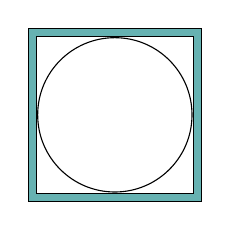
\begin{tikzpicture}
	\draw[fill=teal!60] (-1.1,-1.1) rectangle(1.1,1.1);
	\draw[fill=white] (-1,-1) rectangle(1,1);
	\draw (0,0) circle(.98);
\end{tikzpicture}
\begin{choices}
	\item 在上升过程中，小球对盒子底部有向下的作用力
	\item 在上升过程中，小球对盒子顶部有向上的作用力
	\item 在下降过程中，小球对盒子底部有向下的作用力
	\item 在下降过程中，小球对盒子顶部有向上的作用力
\end{choices}
\begin{answer}
    BC\qquad 提示：
\end{answer}